\documentclass[11pt, oneside]{article} 
\usepackage{geometry}
\geometry{letterpaper} 
\usepackage{graphicx}
	
\usepackage{amssymb}
\usepackage{amsmath}
\usepackage{parskip}
\usepackage{color}
\usepackage{hyperref}

\graphicspath{{/Users/telliott_admin/Tex/png/}}
% \begin{center} 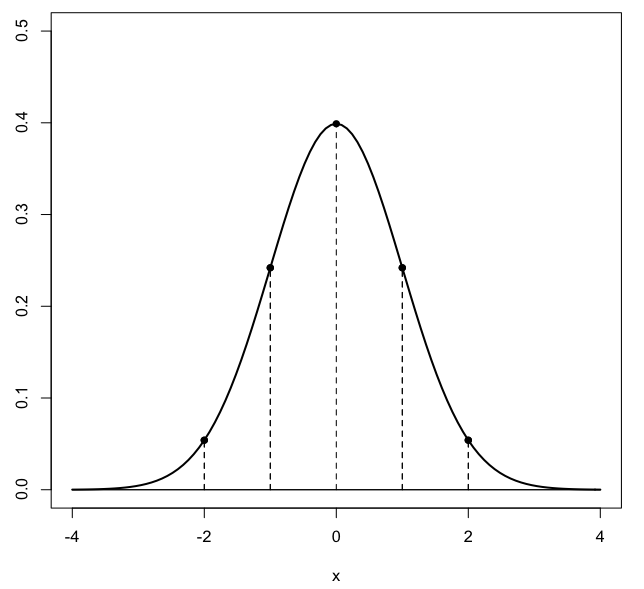
\includegraphics [scale=0.4] {gauss3.png} \end{center}

\title{Field of an infinite sheet}
\date{}

\begin{document}
\maketitle
\Large
Here we evaluate the field at a point a distance $a$ away from an infinite sheet.  The charge density is $\sigma$.  

We start by thinking about a ring with radius $r$ centered on the position that is closest to the point where we're conducting the evaluation.  The normal vector passes through the center of the ring and also through our point.  The distance between them is $x$

\begin{center} 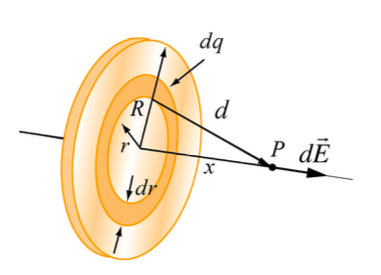
\includegraphics [scale=0.6] {charge_density2.png} \end{center}

The distance between points on the ring and the point where the field is being evaluated is $d$.

The force is directed from each little segment on the ring toward the point, but the part of the force that is not perpendicular is canceled in each case, by an opposite component coming from the piece of the ring on the other side.  So again, we will have a factor of $\cos \theta$.

The relevant distance squared for Coulomb's Law is
\[ d^2 = r^2 + x^2 \]
the factor of $\cos \theta$ is
\[ \cos \theta = \frac{x}{d} = \frac{x}{\sqrt{r^2 + x^2}} \]

So Coulomb says:
\[ dE =  \frac{dq}{4 \pi \epsilon_0} \frac{x}{(r^2 + x^2)^{3/2}} \]

The ring has width $dr$ and length $2 \pi r$, so it has area $2 \pi r \ dr$ and charge $2 \pi r \sigma \ dr$.  We have
\[ dE = \frac{2 \pi r \sigma}{4 \pi \epsilon_0} \frac{x}{(r^2 + x^2)^{3/2}} \ dr \]
\[ dE = \frac{x \sigma}{2 \epsilon_0} \frac{r}{(r^2 + x^2)^{3/2}} \ dr \]
The denominator is similar to what we had in the first problem, but now we have $r \ dr$ up top.

The integral is
\[ E = \int dE = \int \frac{x \sigma}{2 \epsilon_0} \frac{r}{(r^2 + x^2)^{3/2}} \ dr \]
\[ = \frac{x \sigma}{2 \epsilon_0} (-\frac{1}{\sqrt{r^2 + x^2}} ) \]

We evaluate between $r = 0 \rightarrow \infty$.  The term in parentheses becomes $- - 1/\sqrt{x^2}$, so the answer is finally
\[ E  = \frac{\sigma}{2 \epsilon_0} \]

Remarkably, the field is independent of $x$.  If we take a cross-section in the perpendicular plane, the field lines do not spread out.

As before, we can also use Gauss's Law.
\begin{center} 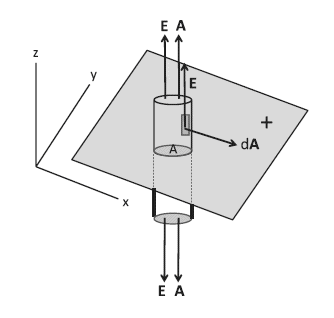
\includegraphics [scale=0.5] {gauss_sheet.png} \end{center}

The Gaussian surface is a cylinder, as shown.  The enclosed charge is $\sigma A$.  Gauss says
\[ \int_S \mathbf{E} \cdot \mathbf{dS} = \frac{Q}{\epsilon_0} =  \frac{\sigma A}{\epsilon_0} \]

Only the end caps of the cylinder intercept any field lines (so the dot product on the curved parts is zero), and for these the field and the normal vector point in the same direction so
\[ \int_S \mathbf{E} \cdot \mathbf{dS} =  E \int dS \]
We must be careful here.  There are \emph{two} end caps
\[ \int dS = 2A \]
\[ = 2A \ E = \frac{\sigma A}{\epsilon_0}  \]
\[ E = \frac{\sigma}{2 \epsilon_0}  \]

\subsection*{sphere}
The problem of the sphere comes up in gravitation as well as electrostatics.  We will sidestep the determination of how a sphere or a solid ball behaves.  (See the chapter on the shell theorem, due to Newton).  We will instead use Gauss's Law, which says the total electric flux through a surface enclosing a charge $Q$ is
\[ \Phi_E = \frac{Q}{\epsilon_0} \]
The flux is defined to be the dot product of the electric field with the surface element, integrated over the entire surface.
\[ \Phi_E = \iint_S \mathbf{E} \cdot d \mathbf{A} \]

If we have a sphere, it is radially symmetric.  Therefore, we expect that the electric field will be perpendicular to the surface of the sphere, and to any (imaginary) sphere that we might draw around the sphere at a radius $r$ from the center.  This means that the dot product is just $E dA$, so
\[ \Phi_E = \iint_S E dA = E \iint_S dA = 4 \pi r^2 E \]
\[ \frac{Q}{\epsilon_0} = 4 \pi r^2 E \]
\[ E = \frac{1}{4 \pi \epsilon_0} \frac{Q}{r^2} \]
\[ \mathbf{E} = \frac{1}{4 \pi \epsilon_0} \frac{Q}{r^2} \ \hat{\mathbf{r}} \]
\[ \mathbf{F} = q\mathbf{E} = \frac{1}{4 \pi \epsilon_0} \frac{qQ}{r^2} \ \hat{\mathbf{r}} \]


\end{document}  